\documentclass{beamer}
\usetheme{metropolis}
\usepackage{graphicx}
\usepackage{subfig}
\usepackage{tcolorbox}
\title{Algebra-Based Physics-2: Electricity, Magnetism, and Modern Physics (PHYS135B-01): Unit 3}
\author{Jordan Hanson}
\institute{Whittier College Department of Physics and Astronomy}

\begin{document}
\maketitle

\section{Unit 2 Review}

\begin{frame}{Unit 2 Summary}
\textbf{Reading: Chapters 20 and 21}
\begin{enumerate}
\item Current, Ohm's Law, resistors and conductors
\item DC circuits I
\item Nerve signals
\end{enumerate}
\end{frame}

\section{Unit 2 Review Problems}

\begin{frame}{Unit 2 Review Problems}
Consider a proton with mass $m$ and charge $q_{\rm p}$.  The proton is located in a region with electric field $E$, and it has initial velocity $v_{\rm i}$ at time $t = 0$.  What is the acceleration of the proton?  What is the proton velocity $v_{\rm f}$ after a time $t$?
\begin{itemize}
\item A: $a = \frac{m}{q_{\rm p}} E$, $v_{\rm f}=v_{\rm i}+t$
\item B: $a = \frac{m}{q_{\rm p}} E$, $v_{\rm f}=v_{\rm i}+\frac{m}{q_{\rm p}} E t$
\item C: $a = \frac{q_{\rm p}}{m} E$, $v_{\rm f}=v_{\rm i}+\frac{q_{\rm p}}{m} E t$
\item D: $a = \frac{q_{\rm p}}{m} E$, $v_{\rm f}=v_{\rm i}+t$
\end{itemize}
\end{frame}

%\begin{frame}{Unit 2 Review Problems}
%Consider a line of charge with linear charge density $\lambda$ C/m, aligned with the z-axis.  What is most likely the expression for the electric field a distance $r$ away from the line?  In this coordinate system, $\phi$ is the angle measured counter-clockwise from the x-axis in the x-y plane, and $z$ is the height above the x-y plane. \textit{Hint: think about symmetry of the charge distribution.}
%\begin{itemize}
%\item A: $\frac{2k\lambda}{r} \hat{r}$
%\item B: $\frac{2k\lambda}{r^2} \hat{r}$
%\item C: $\frac{2k\lambda}{r} \cos\phi \hat{r}$
%\item D: $\frac{2k\lambda}{r} \sin\phi \hat{r}$
%\end{itemize}
%\end{frame}

\begin{frame}{Unit 2 Review Problems}
Consider a 12V battery driving current through a system with a total resistance of $1$ k$\Omega$.  What is the current?  What is the power consumption? 
\begin{itemize}
\item A: 12 mA, 144 W
\item B: 144 mA, 12 mW
\item C: 12 mA, 144 mW
\item D: 14.4 A, 144 W
\end{itemize}
\end{frame}

\section{Summary}

\begin{frame}{Unit 2 Summary}
\textbf{Reading: Chapter 22} \\ \vspace{0.5cm}
\textit{This week: 22.1-22.5}
\begin{enumerate}
\item Magnets and magnetic fields
\item Force on a moving charge in a magnetic field
\item Applications
\end{enumerate}
\textit{This weekend: 22.6-22.10}
\begin{enumerate}
\item The Hall effect
\item Magnetic forces on conductors
\item Torque on a current loop
\item Amp\`{e}re's Law
\end{enumerate}
\end{frame}

\section{Magnets and magnetic fields}

\begin{frame}{Magnets and magnetic fields}
Introductory video on the origin of magnetic fields and forces they exert on charge: \\ \vspace{0.5cm}
\url{https://www.youtube.com/watch?v=s94suB5uLWw}
\end{frame}

\begin{frame}{Magnets and magnetic fields}
What is a cross-product and how does it work? \\ \vspace{0.25cm}
\begin{figure}
\centering
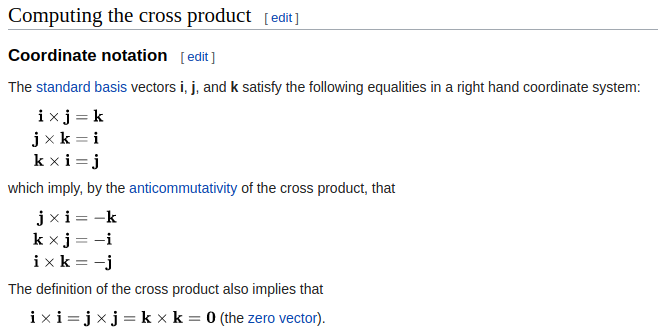
\includegraphics[width=0.75\textwidth]{figures/crossP.png}
\caption{\label{fig:crossP} The cross-product is a way of multiplying unit vectors.}
\end{figure}
\textbf{Professor:} several examples on board.
\end{frame}

\begin{frame}{Magnets and magnetic fields}
Let $\vec{v} = 2\hat{i}$ and $w = -2 \hat{j}$.  What is $\vec{v} \times \vec{w}$?
\begin{itemize}
\item A: $-4 \hat{k}$
\item B: $4 \hat{k}$
\item C: $-2 \hat{i}$
\item D: $2 \hat{j}$
\end{itemize}
\end{frame}

\begin{frame}{Magnets and magnetic fields}
Let $\vec{v} = 3\hat{j}$ and $w = 5 \hat{k}$.  What is $\vec{v} \times \vec{w}$?
\begin{itemize}
\item A: $15 \hat{i}$
\item B: $5 \hat{j}$
\item C: $3 \hat{i}$
\item D: $15 \hat{k}$
\end{itemize}
\end{frame}

\begin{frame}{Magnets and magnetic fields}
Let $\vec{v} = 3\hat{i} \times 3\hat{j}$ and $w = 2 \hat{k}$.  What is $\vec{v} \times \vec{w}$?
\begin{itemize}
\item A: $-6 \hat{j} + 6\hat{k}$
\item B: $-6 \hat{j} + 6\hat{i}$
\item C: $6 \hat{j} + 6\hat{i}$
\item D: $6 \hat{k} + 6\hat{i}$
\end{itemize}
\end{frame}

\begin{frame}{Magnets and magnetic fields}
\textbf{Group exercise:} Compute the following cross product:
\begin{align}
\vec{v} &= 2\hat{i}-2\hat{j} \\
\vec{w} &= 4\hat{j}-4\hat{i} \\
\vec{v} \times \vec{w} &= ??
\end{align}
\end{frame}

\begin{frame}{Magnets and magnetic fields}
\textbf{Group exercise:} Compute the following cross product:
\begin{align}
\vec{v} &= 2\hat{i}-2\hat{j}+\hat{k} \\
\vec{w} &= 4\hat{j}-4\hat{i}-\hat{k} \\
\vec{v} \times \vec{w} &= ??
\end{align}
\end{frame}

\begin{frame}{Magnets and magnetic fields}
\begin{tcolorbox}[colback=white,colframe=black!100!black,title=The Lorentz Force]
\alert{Let a particle with charge $q$ and velocity $\vec{v}$ move through a \textit{magnetic field} $\vec{B}$.  The \textbf{Lorentz force} on the charged particle is
\begin{equation}
\vec{F}_{\rm L} = q\vec{v} \times \vec{B}
\label{eq:Lorentz}
\end{equation}}
\end{tcolorbox}
\textit{As a helpful memory tool, we have the right-hand rule to remember the direction of the cross-product.}  \textbf{The units of the magnetic field are the Telsa}, after Nikola Tesla.  We also have the Gauss which is $10^{-4}$ Tesla.
\end{frame}

\begin{frame}{Magnets and magnetic fields}
\begin{figure}
\centering
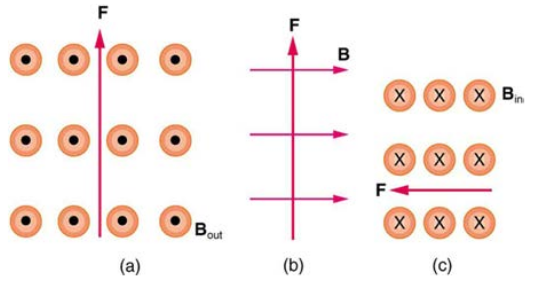
\includegraphics[width=0.75\textwidth]{figures/lorentzProblem.png}
\caption{\label{fig:lorentzProblem} Three different magnetic field and charge scenarios.  The vector $\vec{F}$ is the direction of the Lorentz force, and the magnetic field is uniform.  A dot indicates that the magnetic field is coming out of the page, and an x indicates that the field is going into the page.}
\end{figure}
\end{frame}

\begin{frame}{Magnets and magnetic fields}
\begin{columns}[T]
\begin{column}{0.3\textwidth}
In which of the diagrams is a positively charged particle moving to the left?
\begin{itemize}
\item A: A
\item B: B
\item C: C
\item D: Double WAT
\end{itemize}
\end{column}
\begin{column}{0.7\textwidth}
\begin{figure}
\centering
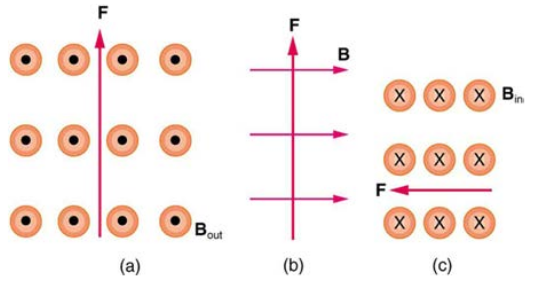
\includegraphics[width=0.75\textwidth]{figures/lorentzProblem.png}
\caption{\label{fig:lorentzProblem2} Three different magnetic field and charge scenarios.}
\end{figure}
\end{column}
\end{columns}
\end{frame}

\begin{frame}{Magnets and magnetic fields}
\begin{columns}[T]
\begin{column}{0.3\textwidth}
In which of the diagrams is a positively charged particle moving upwards?
\begin{itemize}
\item A: A
\item B: B
\item C: C
\item D: Double WAT
\end{itemize}
\end{column}
\begin{column}{0.7\textwidth}
\begin{figure}
\centering
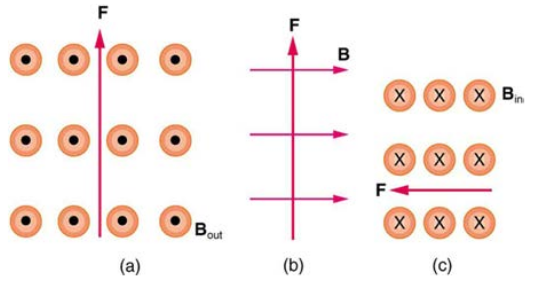
\includegraphics[width=0.75\textwidth]{figures/lorentzProblem.png}
\caption{\label{fig:lorentzProblem3} Three different magnetic field and charge scenarios.}
\end{figure}
\end{column}
\end{columns}
\end{frame}

\begin{frame}{Magnets and magnetic fields}
\begin{columns}[T]
\begin{column}{0.3\textwidth}
In which of the diagrams is a negatively charged particle moving into the page?
\begin{itemize}
\item A: A
\item B: B
\item C: C
\item D: Double WAT
\end{itemize}
\end{column}
\begin{column}{0.7\textwidth}
\begin{figure}
\centering
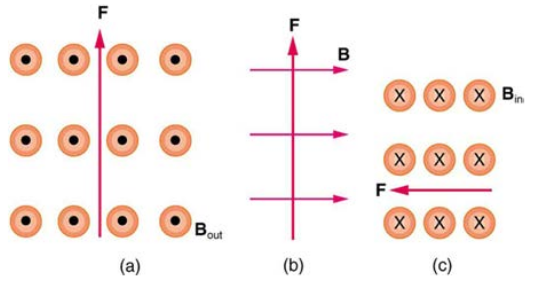
\includegraphics[width=0.75\textwidth]{figures/lorentzProblem.png}
\caption{\label{fig:lorentzProblem4} Three different magnetic field and charge scenarios.}
\end{figure}
\end{column}
\end{columns}
\end{frame}

\begin{frame}{Magnets and magnetic fields}
\begin{columns}[T]
\begin{column}{0.3\textwidth}
In which of the diagrams is a negatively charged particle moving to the right?
\begin{itemize}
\item A: A
\item B: B
\item C: C
\item D: Double WAT
\end{itemize}
\end{column}
\begin{column}{0.7\textwidth}
\begin{figure}
\centering
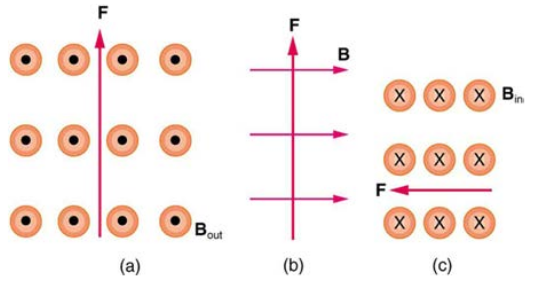
\includegraphics[width=0.75\textwidth]{figures/lorentzProblem.png}
\caption{\label{fig:lorentzProblem5} Three different magnetic field and charge scenarios.}
\end{figure}
\end{column}
\end{columns}
\end{frame}

\begin{frame}{Magnets and magnetic fields}
A theorem for the magnitude of the cross-product:  Let $\vec{a}$ and $\vec{b}$ be vectors and $\theta$ be the angle between them.  The magnitude of the cross-product is
\begin{equation}
|\vec{a} \times \vec{b}| =  a b \sin\theta
\end{equation}
Thus, the magnitude of the Lorentz force is
\begin{equation}
F_{\rm L} = q v B \sin\theta
\end{equation}
The angle $\theta$ is between the velocity and the magnetic field.
\end{frame}

\begin{frame}{Magnets and magnetic fields}
A cosmic ray proton moving toward the Earth at $3 \times 10^{6}$ m/s experiences a magnetic force of $2 \times 10^{-17}$ N. What is the strength of the magnetic field if there is a $45$ degree angle between it and the proton’s velocity?  (Remember that $q$ for a proton is $1.6 \times 10^{-19}$ C).
\begin{itemize}
\item A: 0.1 Gauss
\item B: 0.6 Gauss
\item C: 1 Gauss
\item D: 6 Gauss
\end{itemize}
\end{frame}

\begin{frame}{Magnets and magnetic fields}
\textbf{Other examples:}
\begin{enumerate}
\item Magnetic fields do no work
\item $v = E/B$
\item q/m circle (potential demonstration)
\end{enumerate}
\end{frame}

\begin{frame}{Magnets and magnetic fields}
\begin{figure}
\centering
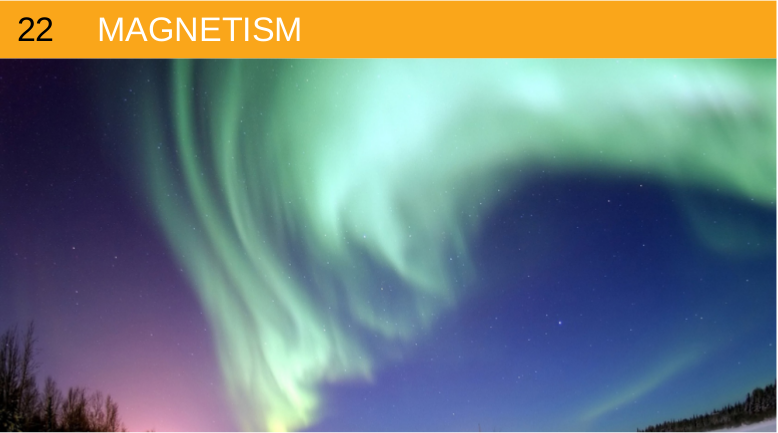
\includegraphics[width=0.9\textwidth]{figures/aurora.png}
\caption{\label{fig:aurora} The aurora borealis, or northern lights.}
\end{figure}
\end{frame}

\begin{frame}{Magnets and magnetic fields}
A cool talk on the aurora borealis:
\url{https://youtu.be/czMh3BnHFHQ} \\
\begin{figure}
\centering
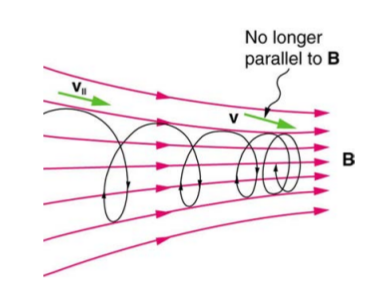
\includegraphics[width=0.45\textwidth]{figures/mag1.png}
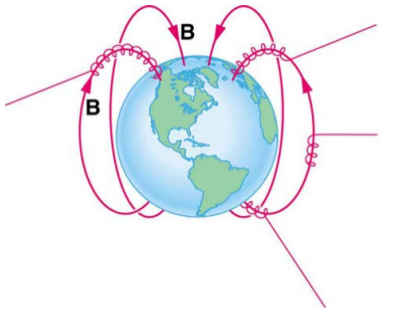
\includegraphics[width=0.45\textwidth]{figures/mag2.png}
\end{figure}
One un-explained piece: what does it mean for the electrons and protons to \textit{high-five} the neutral oxygen and nitrogen atoms?
\end{frame}

\section{The Hall Effect}

\begin{frame}{The Hall Effect}
\begin{figure}
\centering
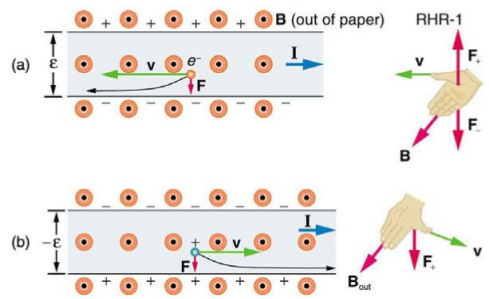
\includegraphics[width=0.6\textwidth]{figures/hall.png}
\caption{\label{fig:hall} Diagram of the Hall effect.  The Hall emf reveals the sign of the moving charges.}
\end{figure}
The Hall emf is 
\begin{equation}
\epsilon = Blv
\end{equation}
The $B$ is the magnetic field, $l$ is the length across the region where charge is flowing, and $v$ is the velocity of the charges.
\end{frame}

\begin{frame}{The Hall Effect}
\textbf{Group board exercise:} Let $n$ be the charge number density in a conductor.  Let $q$ be the charge of an electron.  Let $A$ be the cross-sectional area, and $I$ be the current.  Recall that the \textit{drift velocity of charges in a wire} is given by the equation
\begin{equation}
v_d = \frac{I}{nqA}
\end{equation}
The Hall emf is $\epsilon = Blv$.  Let $v = v_d$, and substitute the first equation into the second equation, and solve for $n$.  Choose reasonable numbers for the current, diameter of a metal wire, and assume a uniform 0.001 T magnetic field is being created around the wire.  Assume a drift velocity of about 1 mm/sec, and solve for $n$.
\end{frame}

\section{Motors}

\begin{frame}{Motors} 
\begin{figure}
\centering
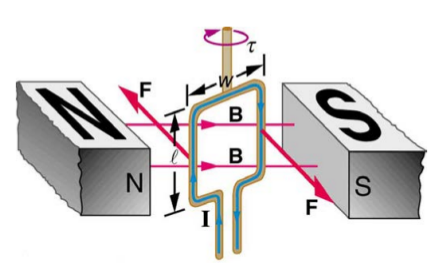
\includegraphics[width=0.6\textwidth]{figures/loop.png}
\caption{\label{fig:loop} In a loop of current in a uniform magnetic field, we find forces going the opposite directions.}
\end{figure}
\end{frame}

\begin{frame}{Motors} 
\begin{figure}
\centering
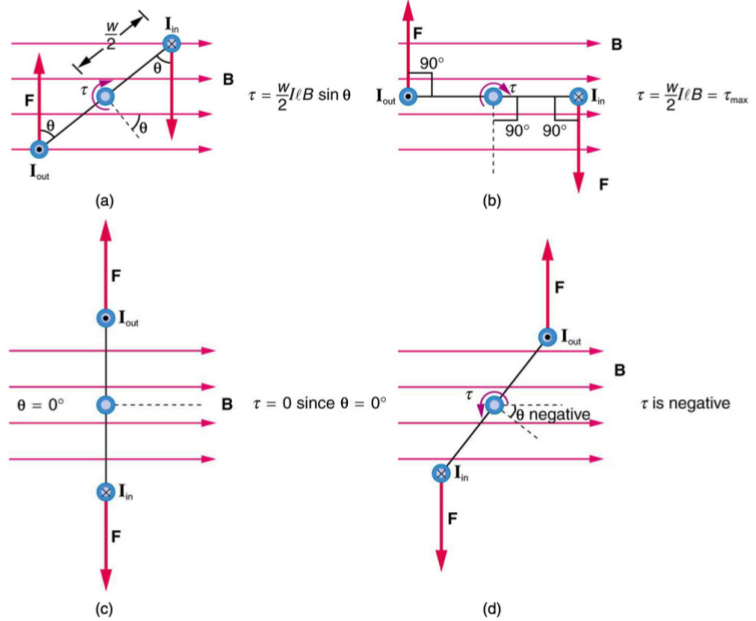
\includegraphics[width=0.6\textwidth]{figures/torque.png}
\caption{\label{fig:loop2} This leads to torque.}
\end{figure}
\end{frame}

\begin{frame}{Motors} 
\begin{figure}
\centering
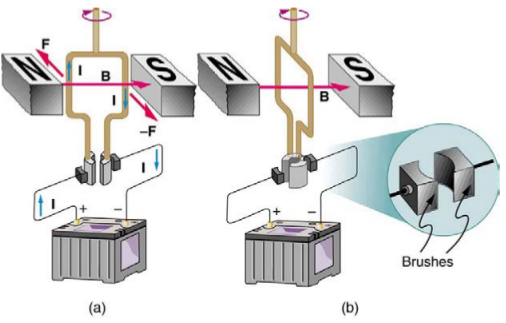
\includegraphics[width=0.6\textwidth]{figures/motor.png}
\caption{\label{fig:loop3} Torque can be used to drive a motor.}
\end{figure}
\end{frame}

\begin{frame}{Motors}
Let the number of loops in the coil be $N$, the current be $I$, the area of the loops be $A$, and the magnetic field be $B$.  The angle between the force and loops is $\theta$.  The magnitude of the torque $\tau$ is
\begin{equation}
\tau = N I A B \sin\theta
\end{equation}
\end{frame}

\begin{frame}{Motors}
At what angle between the loops and the B field is the torque maximized?
\begin{itemize}
\item A: 0 degrees
\item B: 45 degrees
\item C: 90 degrees
\item D: 135 degrees
\end{itemize}
\end{frame}

\begin{frame}{Motors}
Which of the following would boost the torque of a motor?
\begin{itemize}
\item A: Increasing the B-field magnitude
\item B: Decreasing the number of loops
\item C: Increasing the number of loops
\item D: A and C
\end{itemize}
\end{frame}

\begin{frame}{Motors}
Suppose $I = 10$ amps, $B = 0.01$ T, $N = 200$, and the loops have a common radius of 5 cm.  \textbf{Group exercise:} what is the maximum torque?
\end{frame}

\section{Amp\`{e}re's Law}

\begin{frame}{Amp\`{e}re's Law}
\begin{figure}
\centering
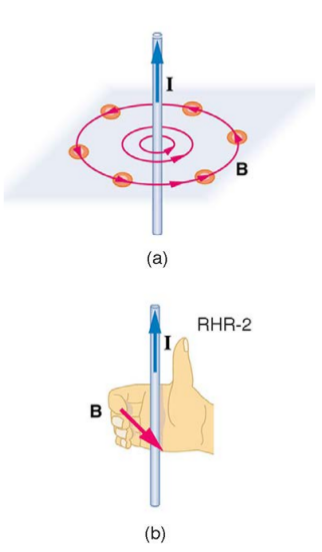
\includegraphics[width=0.3\textwidth]{figures/rhr2.png}
\caption{\label{fig:amp} Magnetic fields creat currents!  To remember the direction, use your right hand.}
\end{figure}
\end{frame}

\begin{frame}{Amp\`{e}re's Law}
Amp\`{e}re's Law states that the current produced by a long straight wire is
\begin{equation}
B = \frac{\mu_0 I}{2\pi r}
\end{equation}
The current is $I$, the distance from the wire is $r$, and $\mu_0 = 4\pi \times 10^{-7}$ T m/A.
\end{frame}

\begin{frame}{Amp\`{e}re's Law}
\textbf{Group exercise:} Suppose we have a wire carrying 1 A, and we are 1 cm away from it.  What is the magnetic field?  What is the magnetic field if another wire is located 1 cm away from us, but carries -1 A? Should the fields add or subtract? \\ \vspace{1cm}
\url{https://youtu.be/1JZLKvWO0ks}
\end{frame}

\begin{frame}{Amp\`{e}re's Law}
\begin{figure}
\centering
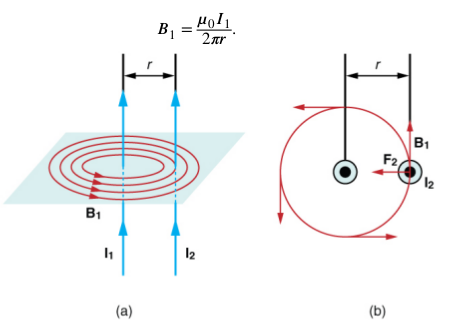
\includegraphics[width=0.5\textwidth]{figures/amp.png}
\caption{\label{fig:amp} Definition of the amp is derived from this setup.}
\end{figure}
\end{frame}

\begin{frame}{Amp\`{e}re's Law}
The B-field at wire 2 due to wire 1 is
\begin{equation}
B_1 = \frac{\mu_0 I_1}{2\pi r}
\label{eq:B}
\end{equation}
The force on wire 2 is 
\begin{equation}
F_2 = I_2 l B_1
\end{equation}
Dividing both sides by $l$ and substituting in Eq. \ref{eq:B}, we have
\begin{equation}
\frac{F}{l} = \frac{\mu_0 I_1 I_2}{2\pi r}
\end{equation}
\textbf{Group board exercise:} let $I_1 = I_2 = 1.0$ A, and $r = 1$ meter.  What is the force per unit length $F/l$?  (Recall that $\mu_0 = 4\pi \times 10^{-7}$ T m/A by definition).
\end{frame}

\section{Magnetic Fields and Work}

\begin{frame}{Magnetic Fields and Work}
Notice from the Lorentz force that magnetic fields do not perform work:
\begin{align}
\vec{F} &= q \vec{v} \times \vec{B} \\ 
\vec{v} t &= \vec{x} \\
\vec{F} &= \frac{q}{t} \vec{x} \times \vec{B} \\
W &= \vec{x} \cdot \vec{F} \\
W &= \frac{q}{t} \vec{x} \cdot \left( \vec{x} \times \vec{B} \right)
\end{align}
\end{frame}

\begin{frame}{Magnetic Fields and Work}
In the final step, why is the right hand side $\left(\vec{x} \cdot \left( \vec{x} \times \vec{B} \right) \right)$ zero?
\begin{itemize}
\item A: Because $\vec{x}$ is parallel to $\vec{x} \times \vec{B}$.
\item B: Because $\vec{x}$ is perpendicular to $\vec{x} \times \vec{B}$.
\item C: Because $q = 0$ on average.
\item D: Because $\vec{x}$ is perpendicular to $\vec{B}$.
\end{itemize}
\end{frame}

\begin{frame}{Faraday and Lenz Laws}
\small
We will continue with the lab activity from last period, in which we began to study how moving magnetic fields \textit{create} emf's (voltages).
\begin{enumerate}
\item Connect the voltmeter and wires to the leads on the set of loops of wire, and obtain a ruler and two bar magnets.
\item The goal is to vary the speed of the magnets through the wire loops:
\begin{itemize}
\item Drop the magnets through the wire loops from different heights about the loops.
\item Make measurements of the initial height of the magnet above the loops.
\item Record the maximum voltage observed as the magnet passes through the loops.
\item \alert{\textbf{Plot the max voltage versus initial height of the magnet, for both polarities of the magnet.}}
\item Repeat with two magnets.
\end{itemize}
\end{enumerate}
\end{frame}

\section{Conclusion}

\begin{frame}{Unit 2 Summary}
\textbf{Reading: Chapter 22}
\begin{enumerate}
\item Magnets and magnetic fields
\item Force on a moving charge in a magnetic field
\item \textbf{The Hall effect}
\item Magnetic forces on conductors
\item \alert{Amp\`{e}re's Law}
\end{enumerate}
\end{frame}

\section{Answers}

\begin{frame}{Answers}
\tiny
\begin{columns}[T]
\begin{column}{0.5\textwidth}
\begin{itemize}
\item $a = \frac{q_{\rm p}}{m} E$, $v_{\rm f}=v_{\rm i}+\frac{q_{\rm p}}{m} E t$
%\item $\frac{2k\lambda}{r} \hat{r}$
\item 12 mA, 144 mW
\item $-4 \hat{k}$
\item $15 \hat{i}$
\item $-6 \hat{j}+6\hat{i}$
\item A
\item C
\item B
\item A
\item 0.6 Gauss
\item 90 degrees
\item A and C
\end{itemize}
\end{column}
\begin{column}{0.5\textwidth}
\begin{itemize}
\item 
\end{itemize}
\end{column}
\end{columns}
\end{frame}

\end{document}
